\documentclass[12pt,a4paper]{report}
\usepackage{geometry}
\geometry{top=14mm, bottom=15mm}
\usepackage[english]{babel}
\usepackage[utf8]{inputenc}
\usepackage{fancyhdr}
\usepackage{csquotes}
\usepackage{listings}
\usepackage{hyperref}
\usepackage{graphics, graphicx}
\usepackage{graphics, graphicx}
\pagestyle{fancy}
\fancyhf{}
%\rhead{}
%\lhead{}
\fancyfoot[LE,LO]{Data Analytics}
\fancyfoot[RE,RO]{Mini Project - 3}
\renewcommand{\footrulewidth}{1pt}
 \medskip
 \author{Abhijeet Singh Panwar (ID : 201351005)}
\title{Data Analytics\\ Mini Project - 3}

\date{\parbox{\linewidth}{\centering%
  \today\endgraf\bigskip
  Instructor : \endgraf\medskip
  Prof. Bhargab Chattopadhyay\endgraf\bigskip
  Indian Institute of Information Technology, Vadodara}}
\begin{document}
\maketitle
\newpage
\section{Question 2}
\textbf{The data below show the sugar content (as a percentage of weight) of several national
brands of children’s and adults’ cereals.}
\\\\
Children’s cereals: 40.3, 55, 45.7, 43.3, 50.3, 45.9, 53.5, 43, 44.2, 44, 47.4, 44, 33.6, 55.1, 48.8, 50.4, 37.8, 60.3, 46.5\\\\
Adults’ cereals: 20, 30.2, 2.2, 7.5, 4.4, 22.2, 16.6, 14.5, 21.4, 3.3, 6.6, 7.8, 10.6, 16.2, 14.5, 4.1, 15.8, 4.1, 2.4, 3.5, 8.5, 10, 1, 4.4, 1.3, 8.1, 4.7, 18.4\\\\
\textbf{Part A}
\\\\
Does it seem reasonable to assume that each sample comes from a normal distribution? Draw Q-Q plots to answer this question.
\\\\
\textbf{Solution}\\\\
QQ-plot is used to check distribution of given data. It uses the information of quantiles of the given data \& compare it with quantiles of other data, whose distribution is already known. In this case, as we are supposed to check whether the given data follows normal distribution or not, we used \texttt{qqnorn}, which take dataset as an input and generate a Q-Q graph. In Q-Q graph, more the data points are in y=x formation , more are the chances of that dataset to follow normal distribution.\\
\begin{center}
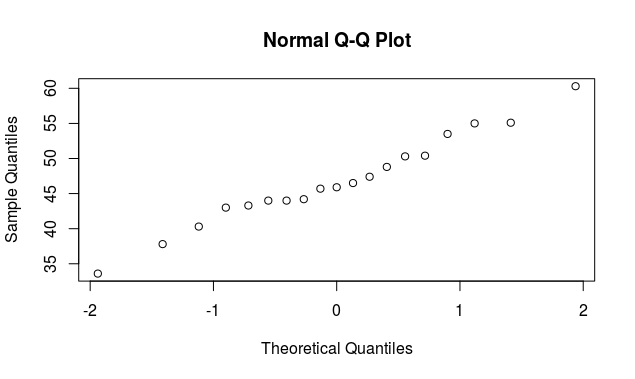
\includegraphics[scale=0.5]{children.png}\\
Q-Q plot for children's cereal data.\\
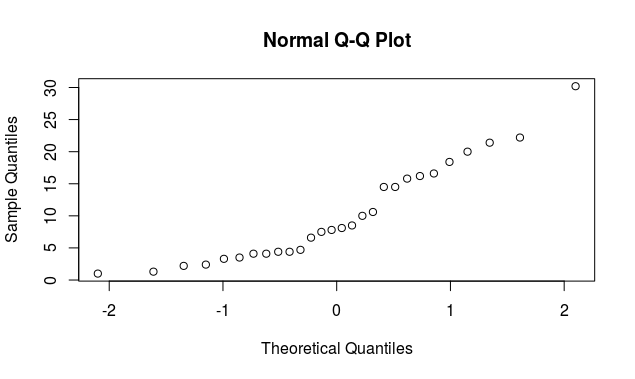
\includegraphics[scale=0.5]{adult.png}\\
Q-Q plot for adult's cereal data.\\
\end{center}
\vspace{0.5 in}
From above image, it is clear that children's cereal data follows normal distribution, whereas adult's cereal data do not.
\\\\
\textbf{Part B}
\\\\
Can the variances of the two distributions be assumed to be equal? Justify your answer.
\\\\
\textbf{Solution}
\\\\
The F hypothesis test is used to test if the variances of two populations are equal. \\In F-test,\\
$H_0 : \lbrace {\sigma_ 1}^2 \rbrace = \lbrace {\sigma _2}^2 \rbrace $\\\\
$H_a : \lbrace {\sigma _1}^2 \rbrace > \lbrace {\sigma _2}^2 \rbrace $ or $\lbrace {\sigma _1}^2 \rbrace  < \lbrace {\sigma _2}^2 \rbrace $or $\lbrace {\sigma _1}^2 \rbrace \neq \lbrace {\sigma _2}^2 \rbrace $\\
\\
Test Statistic:\\\\
F = $\lbrace {s_1}^2 \rbrace \div {s_2}^2$, where are ${s_1}^2$ \& ${s_2}^2$ sample variances.\\\\
Significance Level: $\alpha$ \\\\
Critical Region: The hypothesis that the two variances are equal is rejected if,\\

$F \leq F(1-\alpha \div 2,N_1-1,N_2-1)$, here is the critical value of F-dist. with $N_1-1$ \& $N_2 - 1 $ degrees of freedom and a significance level of $\alpha$ .\\\\
$F \geq F(\alpha \div 2,N_1-1,N_2-1)$\\
\\
In this case,\\\\
F = 0.71\\
$F_1$ = 2.001\\
$F_2$ = 0.47\\\\
Therefore, Variances of children cereal population and adult cereal population are not equal.
\\\\
\textbf{Part C}\\\\
Compute an appropriate 90\% confidence interval for difference in mean sugar contents of the two cereal types. What assumptions did your make, if any, to construct the interval?
\\\\
\textbf{Solution}
\\\\
Assumption $\rightarrow$ Distribution of adult cereal data is also normal.
\\\\
Using the formula,
\begin{center}
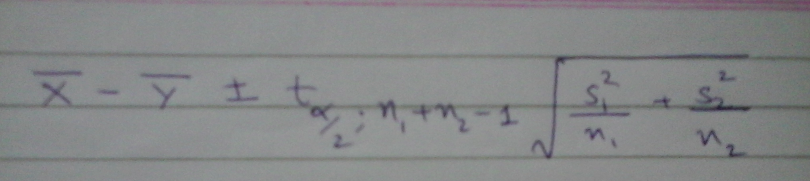
\includegraphics[scale=0.5]{mean.png}
\end{center}
Here,
$\overline{X}$ = mean of children's cereal data\\\\
$\overline{Y}$ = mean of adult's cereal data\\\\
$t_{\alpha \div 2; n_1+n_2-2}$, where $\alpha$ is significance level \& $n_1+n_2$-2 is degree of freedom for t-dist.\\\\
\textbf{Output}\\\\
CI $\rightarrow$ (40.1, 33.18)
\\\\
\textbf{Part D}\\\\
What do you conclude on the basis of your answer in (c)? Can we say that children’s cereals have more sugar on average than adult cereals? If yes, by how much? Justify your answer.
\\\\
\textbf{Solution}\\\\
Based on these samples, with 95\% confidence, children's cereals average between 33.18\% and 40.10\%
more sugar content than adult's cereals.
\\
\newpage
\section{Question 3}
A study shows that 61 of 414 adults who grew up in a single-parent household report that they suffered at least one incident of abuse during childhood. By contrast, 74 of 501 adults who grew up in two-parent households report abuse.\\\\
\textbf{Part A}\\\\
Is there a difference in single-parent and two-parent households when it comes to reporting abuse? Answer this question by computing an appropriate 99\% confidence interval.
\\\\
\textbf{Solution}\\\\
\begin{center}
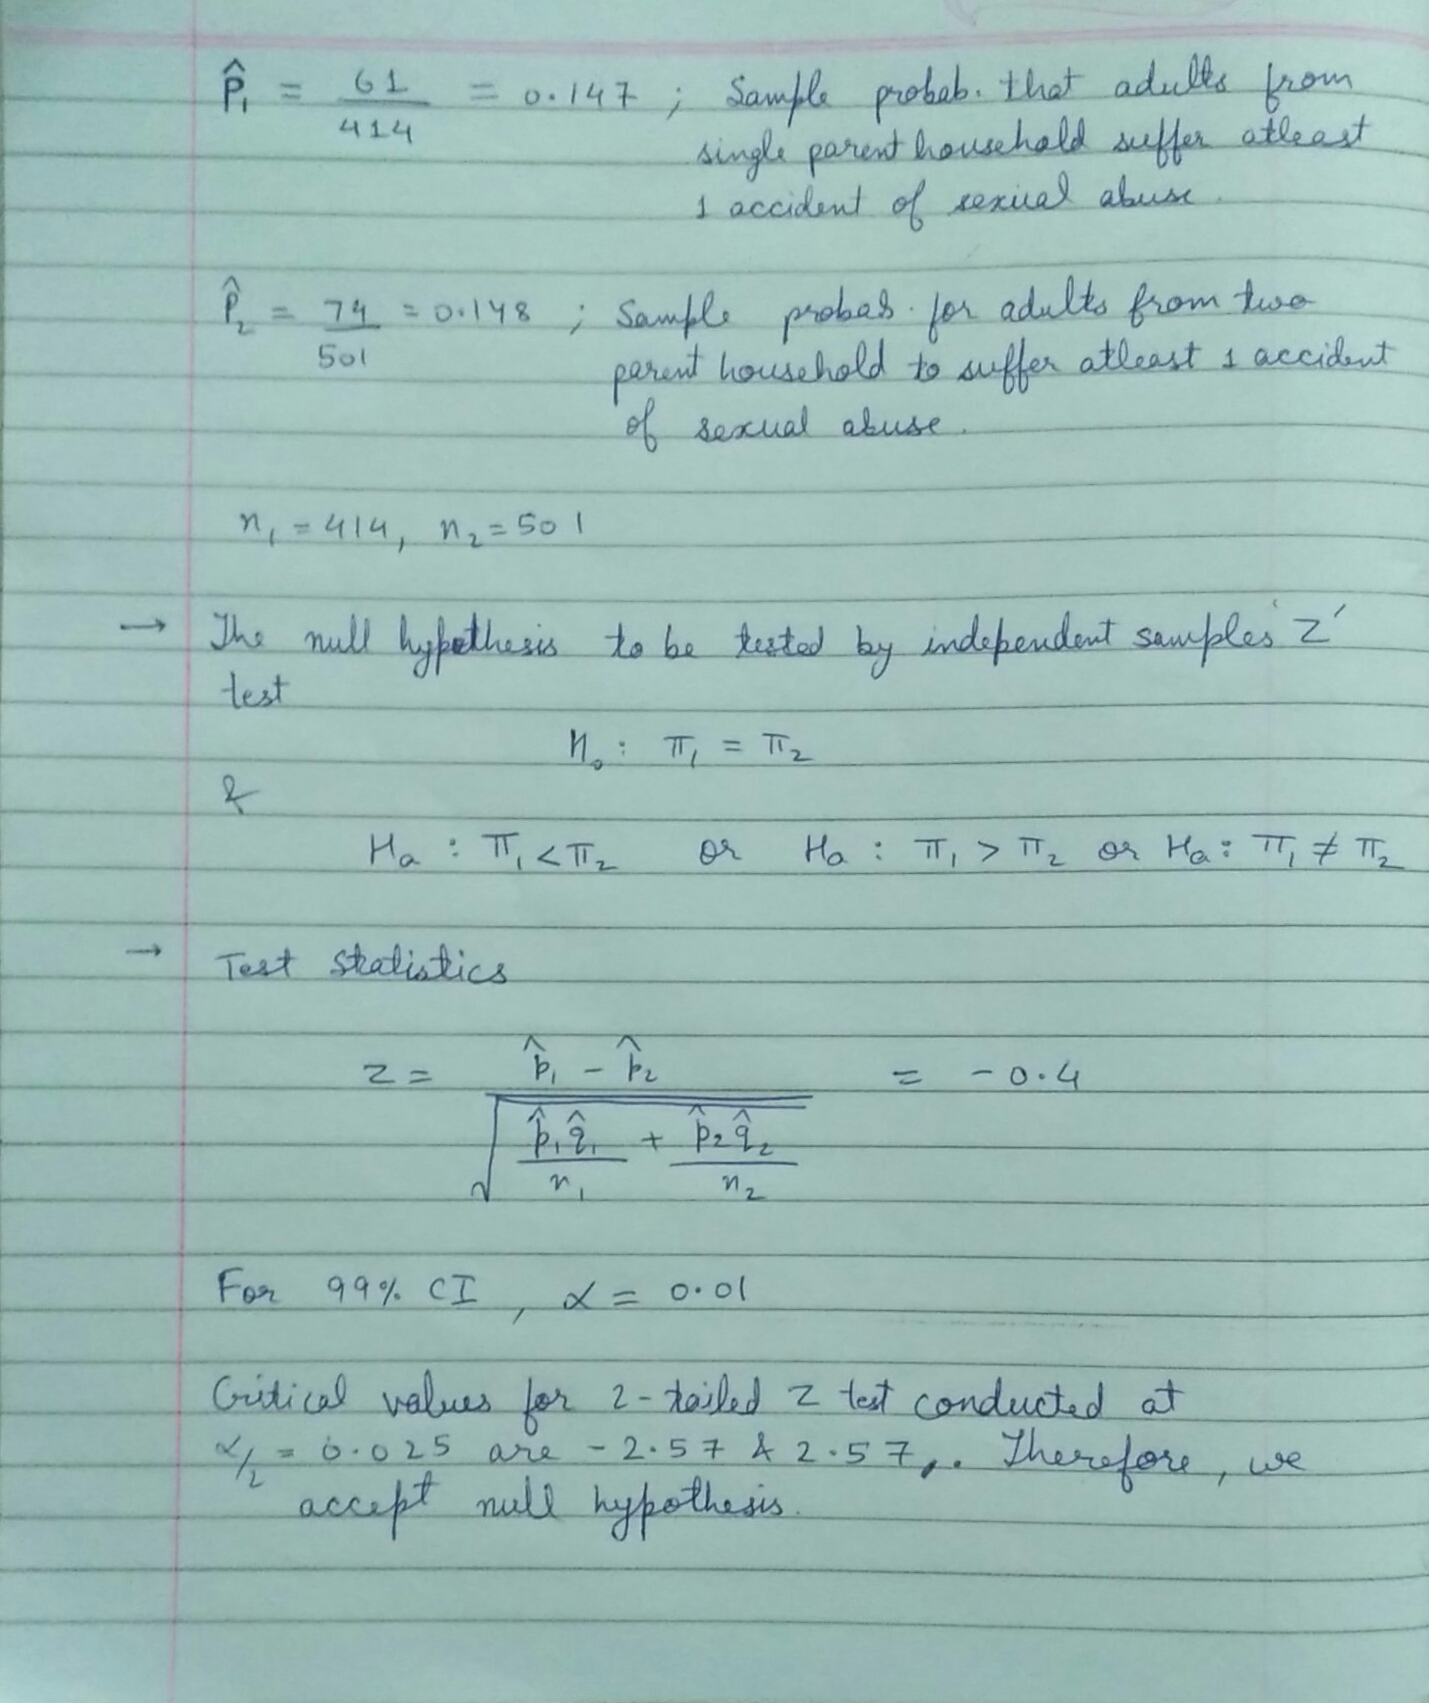
\includegraphics[scale=0.3]{parta.jpg}
\end{center}
\vspace{0.5 in}
\textbf{Part B}\\\\
What assumptions, if any, did you make to compute the interval in (a)? Do the assumptions seem reasonable?\\\\
\textbf{Solution}
\\\\
Use an independent samples Z test for the difference between proportions to test the null hypothesis $H_0 : \Pi 1 = \Pi 2$ against the two-tailed alternative.
\section{R-Code}
\textbf{For Question 1}\\
\begin{lstlisting}

\end{lstlisting}
\textbf{For Question 2}\\
\begin{lstlisting}
#here CI = 90% => alpha = 0.1
#confidence interval for difference in mean sugar contents of the two
#cereal types
#Given: 
#1. both n_1 & n_2 are < 30
#2. var_x & var_y is unknown

#Part A
children = c( 40.3, 55, 45.7, 43.3, 50.3, 45.9, 53.5, 43, 44.2, 44, 47.4, 
44, 33.6, 55.1, 48.8, 50.4, 37.8, 60.3, 46.5)
adult = c(20, 30.2, 2.2, 7.5, 4.4, 22.2, 16.6, 14.5, 21.4, 3.3, 6.6, 7.8, 
10.6, 16.2,14.5, 4.1, 15.8, 4.1, 2.4, 3.5, 8.5, 10, 1, 4.4, 1.3, 8.1, 4.7, 
18.4)
#qqplot to check whether distribution of children cereal & adult cereal is 
#normal or not
qqnorm(children)
qqnorm(adult)

#Assumption
#1. Distribution of adult cereals is also Normal N(u2,s2)
#Module to calculate CI for difference in mean of children & adult cereal

alpha = 0.1 #as CI = 90%
n1 = length(children)
s1 = var(children)#it is square of sd
X = mean(children)

n2 = length(adult)
s2 = var(adult)#it is square of sd
Y = mean(adult)

#B part
#here we use F-test to compare variance of two population
F = s1/s2#generating test statistic
#Calculating critical values
F1 = qf(0.95,n1-1,n2-1)
F2 = qf(0.05,n1-1,n2-1)
if(F<F1 || F>F2)
{print("Variances of children cereal population and adult cereal 
population are not equal")}


#C part
#here qt is used to calculate value of t-dist. given alpha/2 & n1+n2-2 
#as degree of freedom
lowerCI = X-Y-qt(0.05,44)*sqrt((s1/n1)+(s2/n2))
upperCI = X-Y+qt(0.05,44)*sqrt((s1/n1)+(s2/n2))

lowerCI
upperCI
\end{lstlisting}
\end{document}